\section{\textsc{Экспериментальные результаты}}

На панелях (a-с) рис. \ref{fig-ppp-sura} представлены динамики полной ошибки позиционирования в двухчастотном кинематическом режиме PPP для 23 августа 2010 года, 19 и 20 сентября 2016 года, соответственно.
Серые вертикальные полосы означают сеансы работы нагревательного стенда СУРА в эти дни.
Станции упорядочены по мере удаления от стенда сверху (самая ближняя) вниз (самая удалённая). 
Помимо этого, для ближайшей к стенду станции добавлены динамики индекса AATR \cite{Juan2018} (стандартного отклонения производной TEC, нормированной на квадрат наклонного коэффициента) и вариаций TEC с окном фильтрации 10-20 мин, которое было выбрано на основе характерных периодов работы стенда (см. прил. \ref{ap-2}).

На рис. \ref{fig-ppp-sura} (a) обрыв данных для станции ZASU обусловлен отключением электричества.
В целом видно, что уровень ошибки для ZASU выше, чем для других приёмников.
Однако её динамика, как и для других станций, не коррелирует со временем работы стенда, а максимальные значения, наоборот, соответствуют паузе в режиме работы.
Так, для промежутка 12:23-13:00 UT полная ошибка позиционирования достигает 0,5 м, в то время как для остальных станций максимальные значения не превосходят 0,25 м.
Интересно увеличение ошибки на KZN2 в районе 16:40 UT, чего не наблюдается на более близких станциях.
Скорее всего, это просто связано с расходимостью решения PPP.
Также на станции ZASU в районе 17:00 UT возникает резкое увеличение ошибки, которое потом довольно быстро уменьшается, несмотря на наличие ионосферных эффектов в вариациях TEC.
\begin{figure}[h]
\centering    
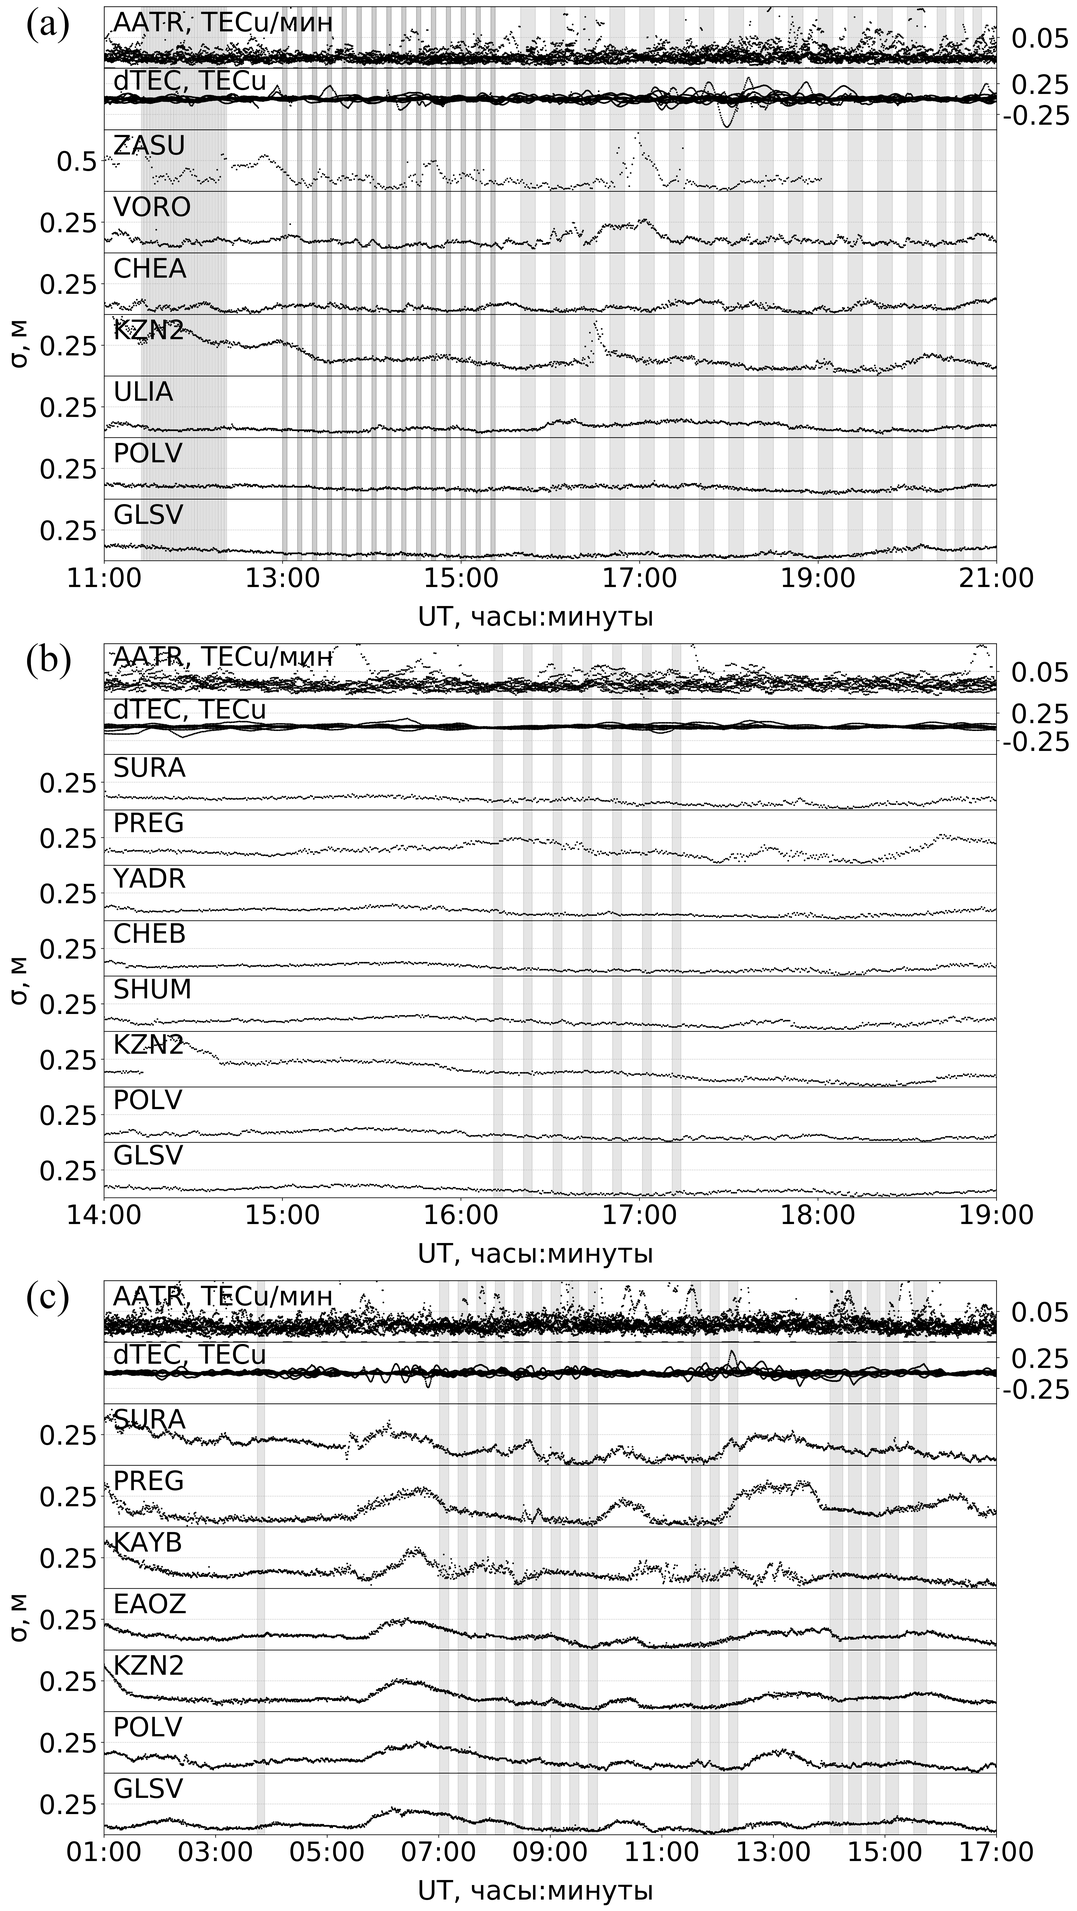
\includegraphics[width=0.75\textwidth]{fig/ppp-sura.png}    
\caption{Динамика полной ошибки позиционирования в двухчастотном кинематическом режиме PPP. (a) -- 23 августа 2010 года, (b) -- 19 сентября 2016 года, (c) -- 20 сентября 2016 года. Серые вертикальные полосы -- сеансы работы нагревательного стенда СУРА. AATR и dTEC -- индекс AATR и вариации TEC с окном фильтрации 10-20 мин для ближайшей к стенду станции, соответственно.}
\label{fig-ppp-sura}      
\end{figure} 
\clearpage

На рис. \ref{fig-ppp-sura} (b) данные показывают отсутствие какого-либо эффекта нагрева.
Ошибка позиционирования остаётся на практически постоянном уровне.
Более того, её значения во время нагрева даже меньше, чем при паузе работы стенда. 
На рис. \ref{fig-ppp-sura} (c) вариабельность ошибки позиционирования больше, чем в другие дни.
Причиной этого может являться более частая смена наблюдаемой группировки спутников.
Таким образом, ни для одного из сеансов работы нагревательного стенда значительного увеличения ошибки позиционирования в режиме PPP зарегистрировано не было.

В табл. \ref{tab-ppp-sura} представлены среднее и среднеквадратическое отклонение (СКО) полной ошибки позиционирования во время сеансов и пауз работы стенда. 
Усреднение производится за весь день.
Интересно, но результаты также показывают более низкие значения ошибки во время нагрева, при этом СКО во время пауз, наоборот, практически всегда больше.
Возможно, это обусловлено разной статистикой. 
\begingroup
\begin{longtable}{|>{\centering\arraybackslash}m{4cm}|c|c|}
\caption{\centerline{Статистика полной ошибки позиционирования PPP.}}
\label{tab-ppp-sura}
\endfirsthead
\endhead
\hline
Станция & \begin{tabular}[c]{@{}c@{}}$\text{Среднее}\pm\text{СКО}$ ошибки \\ во время нагрева, м\end{tabular} & \begin{tabular}[c]{@{}c@{}}$\text{Среднее}\pm\text{СКО}$ ошибки \\ во время пауз, м\end{tabular} \\ \hline
\multicolumn{3}{|c|}{23 августа 2010 года}                                                                                                                                                                       \\ \hline
ZASU    & $0,27\pm0,56$                                                                                       & $0,36\pm0,70$                                                                                    \\ \hline
VORO    & $0,10\pm0,05$                                                                                       & $0,11\pm0,15$                                                                                    \\ \hline
CHEA    & $0,06\pm0,02$                                                                                       & $0,11\pm0,29$                                                                                    \\ \hline
KZN2    & $0,15\pm0,10$                                                                                       & $0,14\pm0,13$                                                                                    \\ \hline
ULIA    & $0,08\pm0,03$                                                                                       & $0,10\pm0,12$                                                                                    \\ \hline
POLV    & $0,09\pm0,02$                                                                                       & $0,14\pm0,21$                                                                                    \\ \hline
GLSV    & $0,06\pm0,03$                                                                                       & $0,10\pm0,13$                                                                                    \\ \hline
\multicolumn{3}{|c|}{19 сентября 2016 года}                                                                                                                                                                      \\ \hline
SURA    & $0,08\pm0,02$                                                                                       & $0,10\pm0,08$                                                                                    \\ \hline
PREG    & $0,13\pm0,06$                                                                                       & $0,15\pm0,15$                                                                                    \\ \hline
YADR    & $0,07\pm0,03$                                                                                       & $0,12\pm0,12$                                                                                    \\ \hline
CHEB    & $0,07\pm0,03$                                                                                       & $0,11\pm0,09$                                                                                    \\ \hline
SHUM    & $0,09\pm0,03$                                                                                       & $0,12\pm0,10$                                                                                    \\ \hline
KZN2    & $0,39\pm0,43$                                                                                       & $0,21\pm0,29$                                                                                    \\ \hline
POLV    & $0,05\pm0,02$                                                                                       & $0,09\pm0,09$                                                                                    \\ \hline
GLSV    & $0,06\pm0,03$                                                                                       & $0,08\pm0,08$                                                                                    \\ \hline
\multicolumn{3}{|c|}{20 сентября 2016 года}                                                                                                                                                                      \\ \hline
SURA    & $0,11\pm0,04$                                                                                       & $0,15\pm0,10$                                                                                    \\ \hline
PREG    & $0,11\pm0,04$                                                                                       & $0,15\pm0,16$                                                                                    \\ \hline
KAYB    & $0,11\pm0,03$                                                                                       & $0,15\pm0,20$                                                                                    \\ \hline
EAOZ    & $0,11\pm0,03$                                                                                       & $0,12\pm0,12$                                                                                    \\ \hline
KZN2    & $0,10\pm0,03$                                                                                       & $0,13\pm0,17$                                                                                    \\ \hline
POLV    & $0,09\pm0,04$                                                                                       & $0,12\pm0,09$                                                                                    \\ \hline
GLSV    & $0,09\pm0,04$                                                                                       & $0,08\pm0,04$                                                                                    \\ \hline
\end{longtable}
\endgroup

В дополнение к двухчастотному кинематическому режиму PPP была рассчитана полная ошибка позиционирования для обычного одночастотного режима по L1C коду. 
Её динамика изображена на рис. \ref{fig-l1c-sura}.
Панелям (a-с) соответствуют 23 августа 2010 года, 19 и 20 сентября 2016 года, соответственно.
В данном режиме реальное состояние ионосферы не учитывается, поэтому ухудшение точности позиционирования из-за активного воздействия более вероятно. 
В целом видно, что уровень ошибки на один-два порядка выше, чем в режиме PPP.
Тем не менее выделить синхронные увеличения, связанные с работой стенда СУРА, не представляется возможным. 
В эксперименте 23 августа 2010 года на рис. \ref{fig-l1c-sura} (a) максимальное ухудшение точности позиционирования ожидалось на станции ZASU в силу её удаления от стенда и расположения антенны (видимая область -- область воздействия).
Однако по итогу даже для этого приёмного пункта не наблюдается видимой связи между динамикой ошибки и временем работы стенда.

В экспериментах 19 и 20 сентября 2016 года на рис. \ref{fig-l1c-sura} (b, c), соответственно, собственные шумы измерений GPS были существенно меньше, чем в эксперименте 2010 года.
Тем не менее на рис. \ref{fig-l1c-sura} (b) видно, что вариации полной ошибки позиционирования для всех станций во время сеансов нагрева не превышают, а в некоторых случаях даже меньше аналогичных вариаций до начала работы стенда. 
На рис. \ref{fig-l1c-sura} (c) также не удаётся выделить однозначной связи с активным воздействием. 
Так, во время первого импульса сеанса 14:01-14:54 UT на станциях KAYB и KZN2 наблюдается резкое увеличения ошибки, которое отсутствует на более близких к стенду приёмных пунктах, а на станции EAOZ, наоборот, имеет место даже уменьшение ошибки. 
\begin{figure}[h]
\centering    
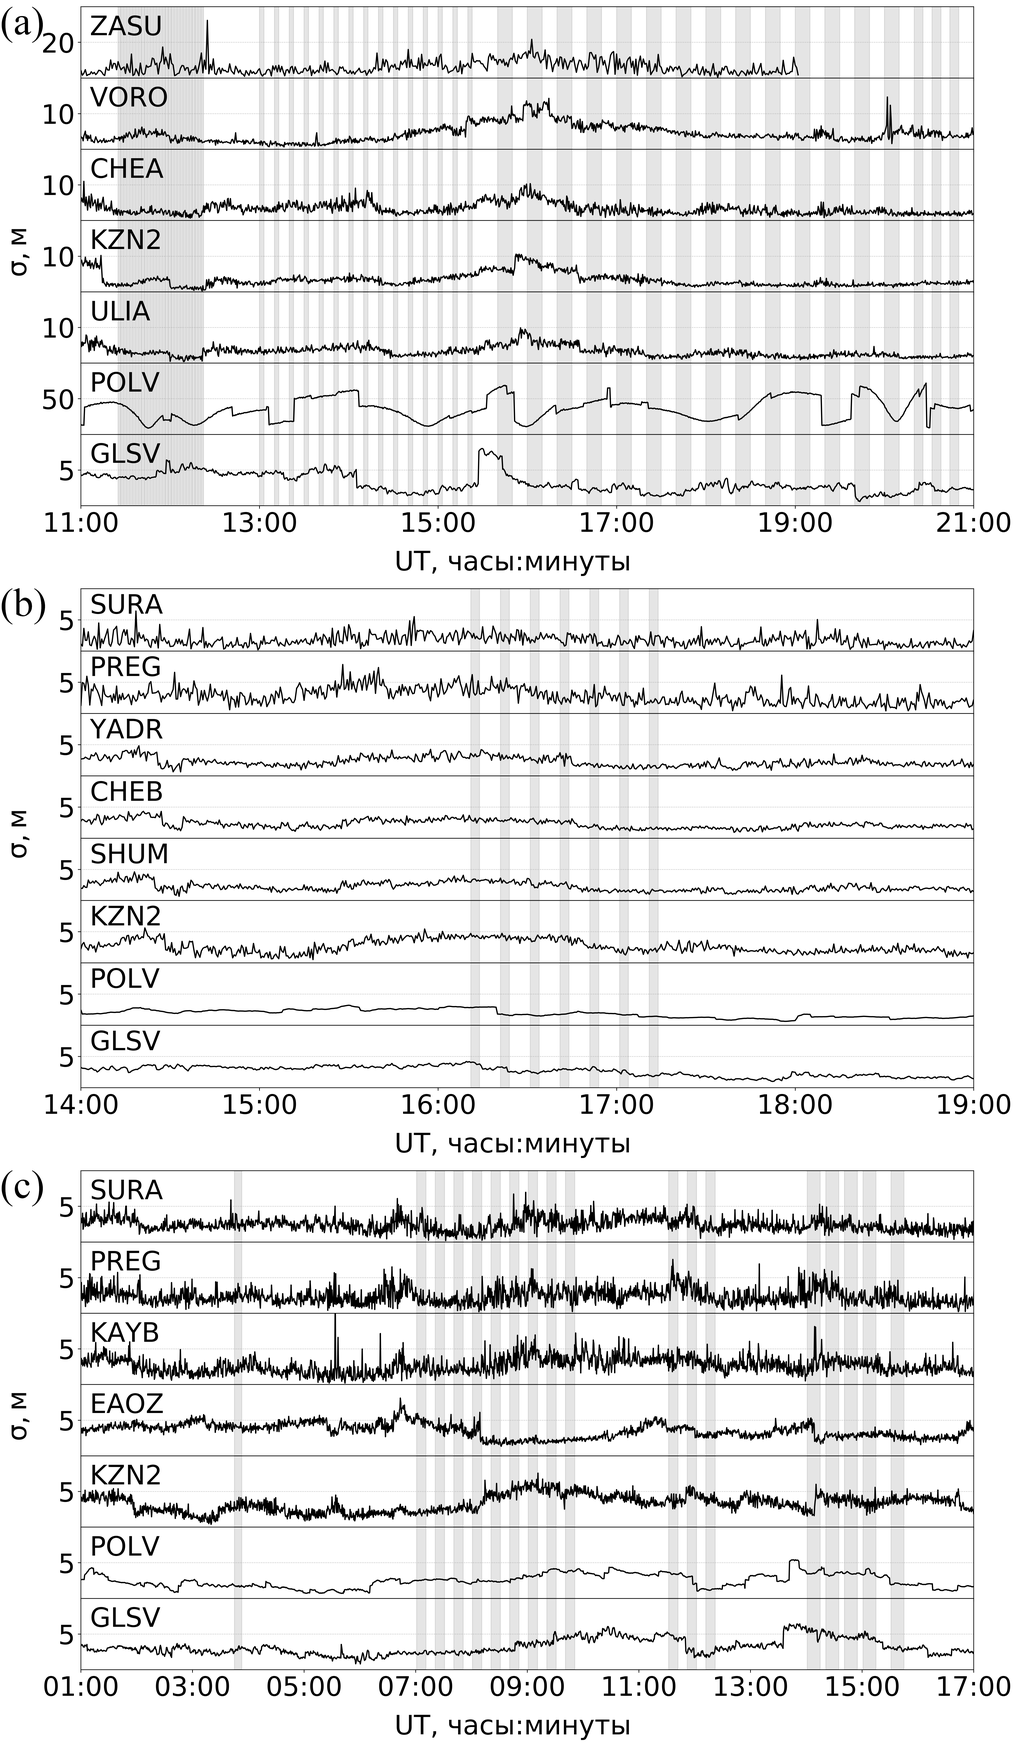
\includegraphics[width=0.75\textwidth]{fig/l1c-sura.png}    
\caption{Динамика полной ошибки позиционирования в одночастотном режиме по L1C коду. (a) -- 23 августа 2010 года, (b) -- 19 сентября 2016 года, (c) -- 20 сентября 2016 года. Серые вертикальные полосы -- сеансы работы нагревательного стенда СУРА.}
\label{fig-l1c-sura}      
\end{figure} 
\clearpage